\documentclass[]{article}
\usepackage{fullpage}
\usepackage{amsmath}
\usepackage{graphicx}
\usepackage{listings}
\usepackage{hyperref}
\usepackage{xcolor}

\title{FOEuler User Guide}
\author{Mianzhi Wang}

\begin{document}

\maketitle

\tableofcontents

\section{Installing FOEuler}

\subsection{System Requirement}
\label{sec:requirement}

FOEuler is a component of the project FOSolverS, which is build upon other open-source packages.
The following tools and packages are required to build FOSolverS:
\begin{itemize}
  \item CMake, the build system used in project FOSolverS
  \item gcc with gfortran, the C and Fortran compiler used in project FOSolverS
  \item an MPI implementation
  \item CGNS, a CFD general notation system
  \item libhdf5, a hierarchical data format library used by CGNS
  \item LAPACK, a dense linear algebra package
  \item SUNDIALS-CVODE, a non-linear stiff ODE solver
  \item libmatheval, a math expression evaluator for UDF
\end{itemize}
In a modern GNU/Linux system distribution, say Ubuntu, all the above required tools and packages can
be installed with the command:
\begin{lstlisting}[backgroundcolor=\color{lightgray}]
  # apt-get install cmake gfortran mpi-default-dev mpi-default-bin \
    libcgns-dev libhdf5-dev liblapack-dev libsundials-serial-dev \
    libmatheval-dev
\end{lstlisting}
Note that the command and the package names may be vary in different GNU/Linux distribution.
If any package is not included the repository of the GNU/Linux distribution on which FOEuler is
deployed, the missing package(s) needs to be manually installed.

Besides the above tools and packages, FOEuler reads unstructured grid generated by GMSH and writes
post-processing data files in the VTK(ParaView) format.
The following command installs these optional external tools:
\begin{lstlisting}[backgroundcolor=\color{lightgray}]
  # apt-get install gmsh paraview
\end{lstlisting}

\subsection{Getting FOEuler}
\label{sec:getting}

The source code of the project FOSolverS is hosted on GitHub.
The home page of the project FOSolverS is \url{https://github.com/mianzhi/fosolvers}.
The full git repository can be downloaded at \\
\url{https://github.com/mianzhi/fosolvers/archive/master.zip}.
In case you are comfortable with git, the version control system used by the project FOSolverS, it
is recommended to clone the full git repository by the following command:
\begin{lstlisting}[backgroundcolor=\color{lightgray}]
  $ git clone https://github.com/mianzhi/fosolvers.git
\end{lstlisting}

\subsection{Building and Installing FOEuler}

The project FOSolverS uses modern build system CMake.
In case that the required packages described in Sec.~\ref{sec:requirement} are properly installed,
and the source are properly downloaded/checked-out as in Sec.~\ref{sec:getting}, the building and
installation of FOEuler is straightforward:
\begin{lstlisting}[backgroundcolor=\color{lightgray}]
  $ cd fosolvers # the top-level CMakeList.txt should be here
  $ mkdir build
  $ cd build
  $ cmake ..
  $ make
  # make install
\end{lstlisting}

\section{Using FOEuler}

\subsection{Overview of the Work Flow}

Figure~\ref{fig:flow} shows the work flow of a simulation with FOEuler.
FOEuler reads grid file ``grid.msh'' in GMSH format.
Boundary conditions, initial conditions, simulation control file, and fluid property file are all
text files.
Their file name must exactly be ``bc'', ``ic'', ``sim'', and ``fl'' respectively.
As the computation runs, post-processing files ``rst\_n.vtk'' (``n'' is an integer starting from 0)
are generated.
These post-processing files can be read by visualization software ParaView.

\begin{figure}[h!]
  \centering
  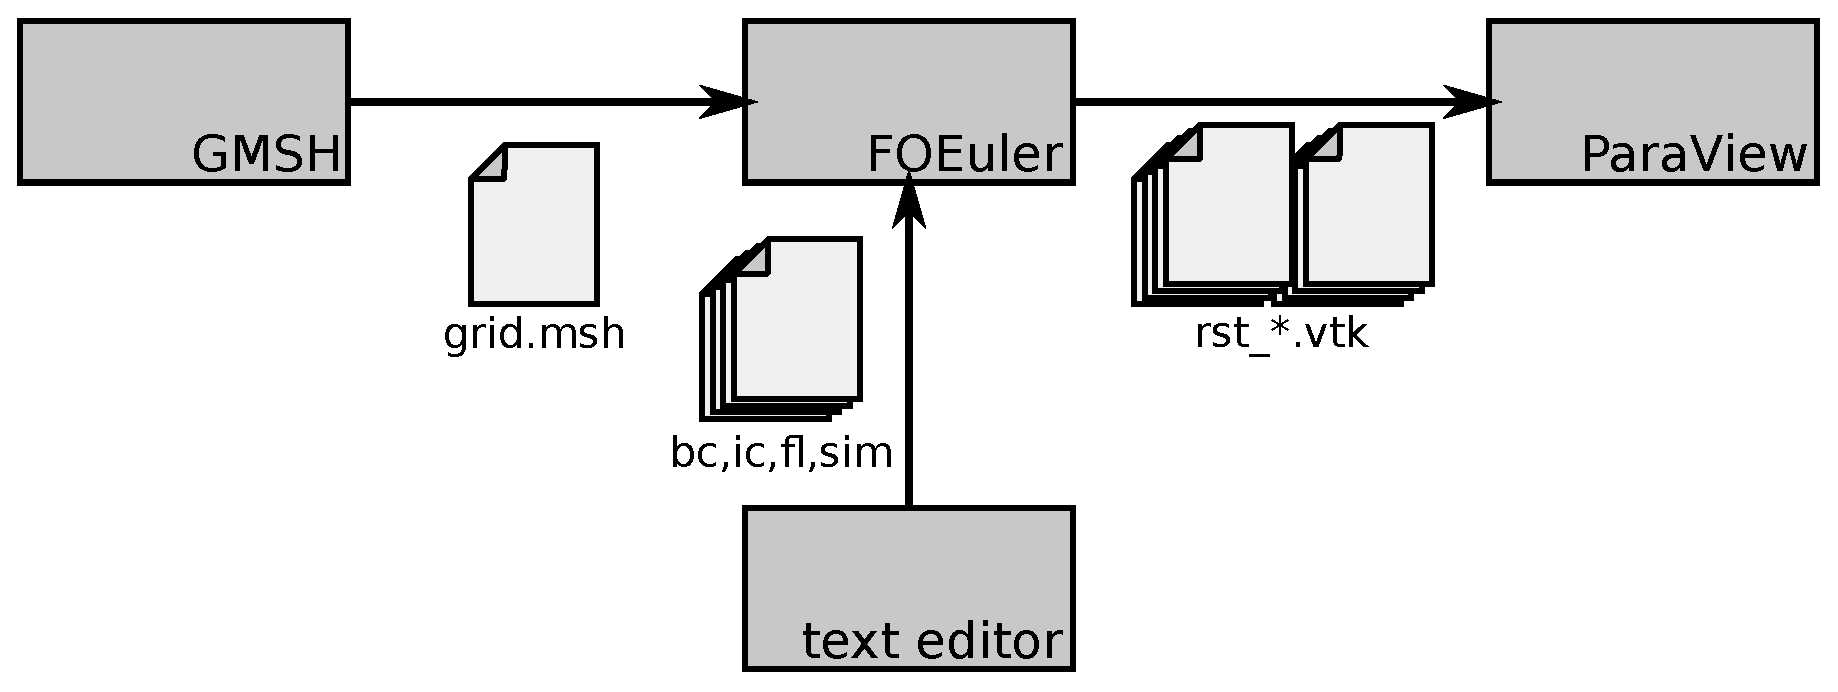
\includegraphics[width=0.7\textwidth]{flow.eps}
  \caption{Work flow of FOEuler simulation.}
  \label{fig:flow}
\end{figure}

\subsection{Preparing Input Files}

\subsubsection{Grid File}
\label{sec:grid}

Preparation of the grid file ``grid.msh'' follows general procedure of grid generation with GMSH.
Note that the GMSH ``geometric entity'' of all the surfaces on which boundary condition are
specified should be recorded.
The value of ``geometric entity'' will be used as ``geometric group identifier'' to associate
boundary condition to a specific surface.

\subsubsection{Simulation Control File}

Figure~\ref{lst:sim} shows an example of simulation control file.
A ``sim'' file consists of two lines, the first line is the total simulation time, the second line
is the time interval between post-processing outputs.

\begin{figure}[h!]
  \begin{lstlisting}[backgroundcolor=\color{lightgray}]
    2e-2	# final time
    5e-4	# output interval
  \end{lstlisting}
  \caption{An example of ``sim'' file.}
  \label{lst:sim}
\end{figure}

\subsubsection{Initial Condition File}

Figure~\ref{lst:ic} shows an example of initial condition file.
The ``ic'' file has five lines, specifying the initial state.
The state variables are static pressure, static temperature, and the three components of velocity.
The initial state is set uniformly through the computation domain according to the given state
variables.

\begin{figure}[h!]
  \begin{lstlisting}[backgroundcolor=\color{lightgray}]
    0.4e5	# initial pressure
    200.	# initial temperature
    350.	# initial velocity, x component
    0.		# initial velocity, y component
    0.		# initial velocity, z component
  \end{lstlisting}
  \caption{An example of ``ic'' file.}
  \label{lst:ic}
\end{figure}

\subsubsection{Boundary Condition File}

Figure~\ref{lst:bc} shows an example of boundary condition file.
The ``bc'' file contains several blocks.
The blocks are separated by exactly one empty line.
The first block has two lines.
The first line specifies the number of boundary conditions, which should equal to the number of the
following blocks.
The second line specifies the maximum number of real parameters for one boundary condition.
The value should be set such that the boundary condition with the largest number of real parameters
does not have more real parameters than this value.
Each following block associates boundary condition for one geometric group, a.k.a. all surfaces with
the same geometric group identifier that are recorded as in Sec.~\ref{sec:grid}.
The geometric group identifier is specified in the first line of each block, followed by another two
integer lines, type of the boundary condition, and the number of real parameters.
The number of real parameters determines the number of real parameter lines of the boundary
condition.
The supported types of boundary condition and required real parameters are shown in
Tab.~\ref{tab:bc}.

\begin{figure}[h!]
  \begin{lstlisting}[backgroundcolor=\color{lightgray}]
    2		# number of conditions
    5		# maximum number of parameters per condition
    
    12		# geometric group identifier
    11		# condition type: inflow with total properties
    5		# number of real parameters
    1.01325e5	# real parameter: total pressure
    300.	# real parameter: total temperature
    382.22	# real parameter: velocity/direction of the flow, x component
    0.		# real parameter: velocity/direction of the flow, y component
    0.		# real parameter: velocity/direction of the flow, z component
    
    1		# geometric group identifier
    20		# condition type: outflow
    1		# number of real parameters
    0.73146e5	# real parameter: static pressure
  \end{lstlisting}
  \caption{An example of ``bc'' file.}
  \label{lst:bc}
\end{figure}

\begin{table}
\caption{All supported boundary conditions.}
  \begin{tabular}{cccl} 
    \hline
    Boundary Type & Code & \# R. Par. & Real Parameters \\ 
    \hline
    Wall & 0 & 0 & N/A \\ 
    In-flow (static) & 10 & 5 &
      static pressure, static temperature, velocity/direction (3 components) \\
    In-flow (total) & 11 & 5 &
      total pressure, total temperature, velocity/direction (3 components) \\
    Out-flow & 20 & 1 & static pressure  \\
    Far-field & 30 & 5 &
      static pressure, static temperature, velocity (3 components) \\
    \hline
  \end{tabular}
  \label{tab:bc}
\end{table}

If any of the surfaces is not explicitly associated with a boundary condition, the wall boundary
condition is used for this surface.

For the two in-flow boundary conditions (static and total), FOEuler computes in-flow Mach number $M$
based on the given in-flow velocity and the thermal state.
In case that $M<1$, the given velocity will be normalized to set the direction of flow, and the
magnitude of the velocity is computed from inside of the domain.

\subsubsection{Fluid Property File}

Figure~\ref{lst:fl} shows an example of fluid property file.
The ``fl'' file has two lines, specifying the mass-specific specific gas constant and the ratio of
heat capacities.

\begin{figure}[h!]
  \begin{lstlisting}[backgroundcolor=\color{lightgray}]
    287.058	# specific gas constant
    1.4		# gamma
  \end{lstlisting}
  \caption{An example of ``fl'' file.}
  \label{lst:fl}
\end{figure}

\subsection{Run FOEuler}

Once all the input files are prepared, the FOEuler solver can be started by:
\begin{lstlisting}[backgroundcolor=\color{lightgray}]
  $ cd my_case # this folder contains all input files
  $ foeuler
\end{lstlisting}
The execution of the program may take a long time depending on the size and nature of the problem.
Post-processing files are generated in the same folder as the solver is running.

\end{document}
